\chapter{Cifrari a blocchi}

I cifrari a blocchi operano su blocchi di $n$ bit di input per produrre 
blocchi di altrettanti $n$ bit in output; la trasformazione deve essere riversibile 
e dipende dalla chiave utilizzata.

\subsubsection{Mappaggi}

Si può pensare di fare un mappaggio tra tutti i possibili blocchi in input 
e il corrispondente cifrato, che deve essere unico; facendo questo 
mappaggio il numero di trasformazioni possibili è $2^n$

\begin{figure}[H]
    \centering
    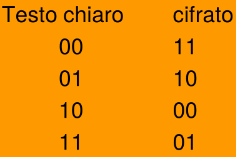
\includegraphics[width=0.3\linewidth]{chapters/chap03/images/mappaggi.png}
\end{figure}

\noindent Il problema è che per blocchi di piccole dimensioni equivale a fare una 
cifratura a sostituzione (vulnerabile ad analisi statistica), mentre per blocchi grandi 
diventa un problema la gestione della chiave: \textbf{per blocchi di n bit la chiave è di dimensione 
$n*2^n$} (la chiave equivale alla tabella delle sostituzioni).

\section{Cifratura di Feistel}

L'idea è quella di approssimare un sistema ideale di cifratura, facendo uso di cifrature in sequenza 
per ottenerne una più complessa rispetto ad una singola trasformazione.

\noindent La chiave scelta permette di calcolare per ogni blocco di input uno di output; è 
una trasformazione robusta dato che è difficile da invertire se non si conosce la chiave.

\subsection{Principi di Shannon}
Feistel alterna \textbf{permutazioni} e \textbf{sostituzioni}; applicano i principi di Shannon 
per contrastare l'analisi statistica:
\begin{itemize}
    \item \textbf{Diffusione:} ogni bit del cifrato dipende da più bit in chiaro; viene estesa la correlazione 
    statistica, non c'è correlazione $1:1$
    \item \textbf{Confusione:} si vuole aumentare la difficoltà nel capire la correlazione tra 
    testo in chiaro/cifrato e la chiave; è reso possibile dal fatto che dalla chiave vengono 
    generate più sottochiave, per un cui un cambiamento di un singolo bit della chiave genera cambiamenti a cascata 
    su tutte le sottochiavi e il cifrato
\end{itemize}

\subsection{Struttura di Feistel}

\begin{itemize}
    \item Blocchi e chiave di grande dimensioni aumentano la sicurezza ma diminuiscono le prestazioni
    \item Tutte le fasi hanno la stessa struttura 
    \item A partire dalla chiave vengono prodotte tante sottochiavi quanti sono i \textit{round}
    \item La funzione di round deve essere non lineare (altrimenti sarebbe facilmente invertibile)
\end{itemize}

\noindent La struttura di Feistel è la seguente:

\begin{figure}[H]
    \centering
    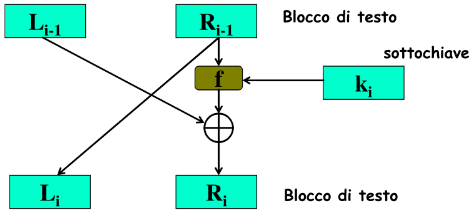
\includegraphics[width=0.8\linewidth]{chapters/chap03/images/feistel.png}
\end{figure}

Il blocco di input viene diviso in due (\textit{left} e \textit{right}), e l'output viene 
ottenuto secondo la procedura mostrata in figura.

\noindent Questa operazione viene ripetuta per tutti i blocchi, per implementare i principi di Shannon.

\noindent È da notare come viene sfruttata la proprietà dello XOR per cui è possibile decifrare 
a prescindere della funzione $f$ utilizzata.

\begin{itemize}
    \item \textbf{Cifratura:} basta implementare un solo round, che verrà ripetuto su tutti i blocchi 
    \item \textbf{Decifratura:} usa lo stesso algoritmo ma con le sottochiavi in ordine inverso 
\end{itemize}

\section{DES}

\begin{figure}[H]
    \centering
    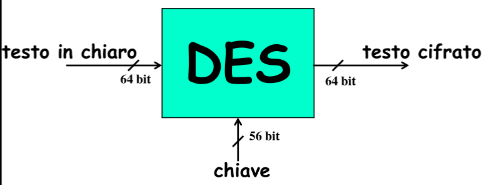
\includegraphics[width=0.8\linewidth]{chapters/chap03/images/des.png}
\end{figure}

Usa la struttra di Feistel, con:
\begin{itemize}
    \item blocchi di 64 bit 
    \item chiave di 64 bit, di cui 56 usati effettivamente dall'algoritmo
    \begin{itemize}
        \item l'ultimo bit di ciascun byte viene usato come bit di parità (è lo XOR dei 7 precedenti)
        \item spazio delle chiavi di $2^{56}$
    \end{itemize}

\end{itemize}

\subsection{Struttura di DES}

\begin{figure}[H]
    \centering
    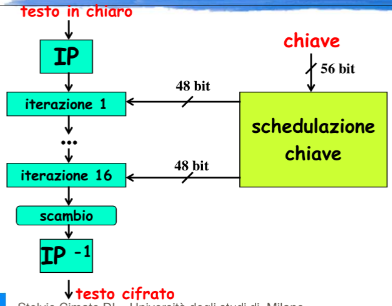
\includegraphics[width=0.7\linewidth]{chapters/chap03/images/des2.png}
\end{figure}

\subsubsection{IP e IP$^{-1}$}

Una permutazione iniziale ed inversa alla fine; usano tabelle fissate per fare 
permutazioni dei bit.

\subsubsection{Singola iterazione}

\begin{figure}[H]
    \centering
    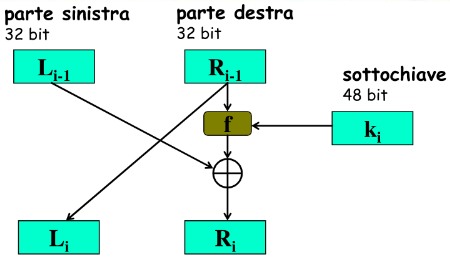
\includegraphics[width=0.7\linewidth]{chapters/chap03/images/des3.png}
\end{figure}

\subsubsection{La funzione $f$}

\noindent I 32 bit di input vengono espansi a 48, e poi vengono messi in XOR con la chiave.

\noindent I 48 bit risultanti vengono gestiti da 8 \textbf{\textit{S-Box}} (6 bit ciascuna), ciascuna delle quali produce 
4 bit per otterne 32; questi 32 bit vengono dati ad una funzione di permutazione e si ottiene il risultato finale.

\begin{figure}[H]
    \centering
    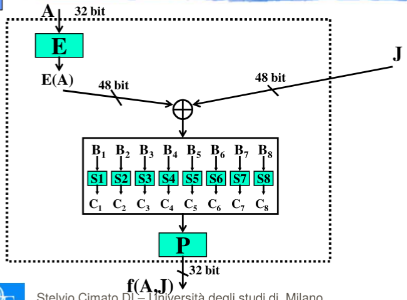
\includegraphics[width=0.7\linewidth]{chapters/chap03/images/f.png}
\end{figure}

\subsubsection{S-Box}

I 6 bit dati in input alle s-box fungono da indici di riga e di colonna per una tabella 
contenente tutti i possibili 16 valori dei 4 bit di output 

\begin{figure}[H]
    \centering
    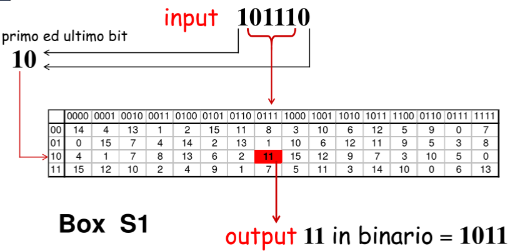
\includegraphics[width=0.7\linewidth]{chapters/chap03/images/s-box.png}
\end{figure}

\noindent Le s-box hanno due proprietà importanti:
\begin{itemize}
    \item cambiando un solo bit di input variano almeno due bit nell'output 
    \item il numero di input per il quale il bit di output è 0 o 1 è circa lo stesso
\end{itemize}


\subsection{Decifratura}

Funziona allo stesso identico modo, ma usando l'ordine inverso delle sottochiavi.

\begin{figure}[H]
    \centering
    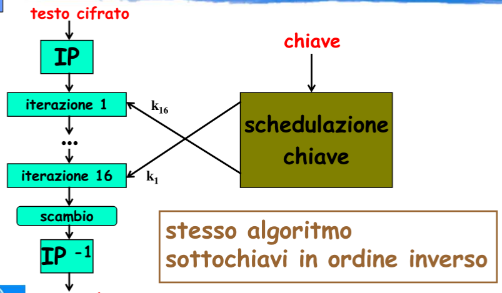
\includegraphics[width=0.8\linewidth]{chapters/chap03/images/des4.png}
\end{figure}

\subsection{Caratteristiche di DES}

Cosidetto \textbf{effetto valanga:} piccoli cambiamenti nel testo in chiaro 
provocano un grande cambiamento nel cifrato; lo stesso vale per la chiave e l'algoritmo 
di schedulazione.

\noindent Rende difficile per un attaccante fare delle analisi tra i bit input e di output.

\subsection{Modalità operative}

Fino ad ora abbiamo visto come viene cifrato un singolo blocco; ora vediamo le modalità 
con cui cifrare più blocchi. Sono valide per tutti i cifrari simmetrici.

\begin{itemize}
    \item \textbf{Electronic Codebook Chaining (ECB):} ciascun blocco di 64 bit viene 
    cifrato in maniera indipendente; ha il vantaggio di evitare la propagazione degli errori ma ha 
    il problema di essere deterministico (a stesso blocco e chiave, corrisponde semmpre lo stesso output); non 
    è sicuro se usato con messaggi lunghi

    \item \textbf{Cipher Block Chaining (CBC):} l'input si ottiene facendo lo XOR con il precedente 
    blocco cifrato; per il primo blocco si usa un \textit{inizialization vector} da scegliere in modo casuale;
    c'è propagazione degli errori ma la cifratura non è più deterministica

    \begin{figure}[H]
        \centering
        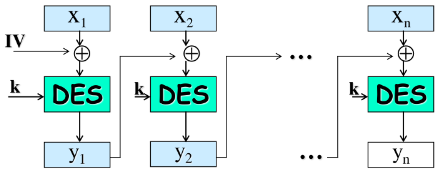
\includegraphics[width=0.6\linewidth]{chapters/chap03/images/cbc.png}
    \end{figure}

    \item \textbf{Cipher Feedback (CFB):} viene usato un registro a scorrimento che permette di poter 
    usare la lunghezza del blocco a piacere; usa sempre un $iv$ per rompere il determinismo, ha propagazione 
    degli errori; l'idea è quella di avvicinarsi ad un cifrario a flusso dato che si può scegliere la lunghezza del 
    blocco a piacere 

    \item \textbf{Output Feedback (OFB):} ha il vantaggio di non propagare gli errori di trasmissione 
    dei bit (usato ad esempio per trasmissione con i satelliti); ha lo svantaggio di essere più 
    vulnerabile ad una modifica del flusso 

    \item \textbf{Counter (CTR):} si usa un contatore delle dimensioni del blocco in chiaro; per ogni 
    blocco successivo il contatore viene incrementato

    \begin{figure}[H]
        \centering
        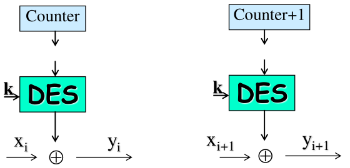
\includegraphics[width=0.6\linewidth]{chapters/chap03/images/ctr.png}
    \end{figure}

    \noindent Ha il vantaggio di essere sicuro ed efficiente

\end{itemize}

\subsection{Crittoanalisi}

Avendo una chiave di 56 bit DES è vulnerabile ad un attacco di brute force. 

\begin{itemize}
    \item La modalità ECB, essendo deterministica, non è resistente al CPA 
    \item Le altre modalità sono tutte resistenti a CPA, dato che l'$iv$ introduce 
    un fattore di casualità
    \item Rimangono comunque degli schemi vulnerabili al CCA 
\end{itemize}

\noindent Alcune tecniche di crittoanalisi (applicabili a tutti i cifrari a blocchi) sono:
\begin{itemize}
    \item crittoanalisi differenziale $\rightarrow$ CPA, anche se necessita di $2^{47}$ 
    testi in chiaro (poco applicabile nella realtà)
    \item crittoanalisi lineare $\rightarrow$ KPA, poco applicabile perché necessita di $2^{43}$ testi noti
\end{itemize}


\section{DES doppio}

Consiste nel cifrare due volte, applicando DES con due chiavi distinte. 

\begin{figure}[H]
    \centering
    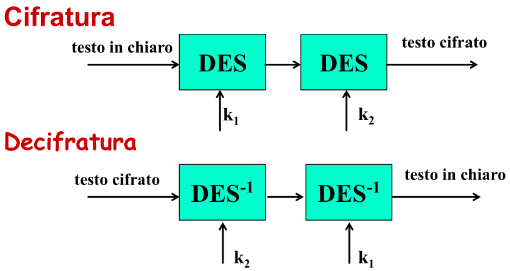
\includegraphics[width=0.8\linewidth]{chapters/chap03/images/des-d.png}
\end{figure}

\noindent È dimostrato che l'insieme delle permutazioni delle chiavi DES non 
è chiuso per composizione, ovvero che non sempre esiste una chiave $k_3 \equiv k_1 \cdot k_2$ (nel 
senso che dà in output lo stesso cifrato della doppia cifratura).

\subsection{Attacco \textit{meet in the middle}}

È un attacco di tipo \textit{known plaintext}.

\noindent Data una coppia nota $(m, c)$ vengono eseguite tutte le cifrature 
per tutti i possibili $2^{56}$ valori di $k_1$, e memorizzate in una tabella.

\noindent Vengono eseguite tutte le possibili decifrature per i $2^{56}$ possibili 
valori di $k_2$, e si cerca una corrispondenza nella tabella.

\noindent Anche se si ha uno spazio delle chiavi delle chiavi di $2^{112}$, la complessità computazionale 
rimane di $2^{56}$; lo stesso vale in termini di spazio per salvare le righe 
della tabella.

\section{DES-X}


È una tipologia di DES che usa una tecnica detta \textit{key withening} per migliorare la sicurezza rispetto al DES classico. 

\noindent In questo
caso, il cifrario non viene rafforzato contro attacchi analitici (analisi differenziale e lineare), ma solo contro gli attacchi
a forza bruta. Vengono applicati due XOR prima e dopo l’esecuzione dell’algoritmo DES con due chiavi aggiuntive
(una per XOR): $DES-X(M)=k_2 \oplus DES(M \oplus k_1)$ 


\section{Blowfish}

È un cifrario che utilizza diverse tecniche tra cui la rete di Feistel e s-box dipendenti 
dalla chiave, cosa che lo rende uno degli algoritmim più sicuri in circolazione. 

\noindent I blocchi hanno una dimensione di 64 bit, mentre la chiave va dai 32 ai 448 bit.

\noindent L'algoritmo consiste in due fasi:
\begin{enumerate}
    \item \textbf{Espansione della chiave:} la chiave viene espansa in 18 sottochiavi a 32 bit e vengono 
    generate 4 s-box dipendenti da essa 
    \item \textbf{Cifratura:} sono previsti 16 round dove in ognuno viene usata una sottochiave; al termine 
    dei round vengono usate le ultime due chiavi rimaste; la decifrazione funziona allo stesso modo 
    ma usando le sottochiavi in ordine inverso
\end{enumerate}

\noindent Questo algoritmo è compatto e veloce; è inoltre resistente agli attacchi di forza 
bruta dato che è possibile arrivare ad uno spazio delle chiavi di $2^{448}$


\section{AES}

Non è un cifrario di Feistel, ma opera in parallelo sull'intero blocco 
di input.
\begin{itemize}
    \item blocchi e chiave da 128 bit 
    \item 10 round 
    \item vengono schedulate 44 sottochiavi a 32 bit 
\end{itemize}

\noindent L'unità di base di AES è il byte; viene rappresentato sotto forma di una matrice 
$4x4$, che prende il nome di \textit{stato}; tutte le operazioni prendono e restituiscono un byte, definendo 
un campo finito su valori fino a $2^8$.

\noindent Ogni round è una composizione parallela di 4 operazioni, che prendono 
in input la matrice di stato:
\begin{itemize}
    \item \textbf{SubBytes}
    \item \textbf{ShiftRows}
    \item \textbf{MixColumns}
    \item \textbf{AddRound Key}
\end{itemize}

\noindent Fanno eccezione una \textit{AddRound Key} prima dei round, e l'ultimo 
dove manca la \textit{MixColumns}.



\subsubsection{SubBytes}

Viene fatta la sostituzione dei byte con un altri, mediante un s-box tabellare, 
costruita in modo da resistere alla crittoanalisi.

\subsubsection{ShiftRows}

Viene fatto uno shift delle righe:
\begin{itemize}
    \item la seconda shiftata di 1 
    \item la terza shiftata di 2 
    \item la quarta shiftata di 3
\end{itemize}

\noindent In questo modo con questa semplice permutazione i 4 byte di una 
colonna vengono riposizionati su colonne differenti.

\subsubsection{MixColumns}

Una colonna viene moltiplicata per un polinomio fissato, viene fatta una combinazione 
lineare.

\subsubsection{AddRoundKey}

Viene fatto lo XOR tra una colonna e la sottochiave di round.

\section{Considerazioni sulla sicurezza}

Ciò che viene fatto con i cifrari a blocchi è mettere il risultato 
in XOR con il successivo \textit{plaintext}; è un modo per approssimare il 
cifrario perfetto dove si ha una chiave casuale lunga quanto il messaggio (sicurezza 
perfetta).

\noindent Usare i cifrari a blocchi in questo modo consente di ottenere 
un flusso di bit che si avvicina ad essere casuale; si sta approssimando OTP con 
64 bit (DES) e 128 bit (AES).

\noindent Come operazione viene usato lo XOR perché non permette di trarre alcuna 
informazione osservando il cifrato.




